
\documentclass{article}
\usepackage{authblk}
\usepackage{graphicx}

\setlength{\parskip}{1.5em}
\setlength{\parindent}{0em}
\renewcommand{\baselinestretch}{1}
\usepackage[paperheight=11.69in,paperwidth=8.27in,left=1.0in,right=1.0in,top=1.6in,bottom=1.7in,headheight=1in]{geometry}

\title {\textbf{Introduction to Bayesian network and its application in prediction coronary heart disease}}
\author[a]{Hao Ying}
\affil[a]{Department of Biostatistics, School of Public Health Science, University of Miami, USA}
\date{}
\renewcommand\Affilfont{\itshape\small}


%%% TEXT  BEGINS  HERE %%%
%%%%%%%%%%%%%%%%%%%%%%%%%%%%%%

\begin{document}
%%%   FACE   %%%%%%%%%%%%%%%%%%%%%%%%%%%%%%
\maketitle





%%%   INTRODUCTION   %%%%%%%%%%%%%%%%%%%%%%%%%%%%%%
\section{INTRODUCTION}
\subsection{Bayesian network}
Bayesian network (BN) is a probabilistic graphical model that represents a set of variables and their conditional dependencies via a directed acyclic graph (DAG). Bayesian networks are ideal for taking into account the prior knowledge about the data structure and use it to study the likelihood of the components of interest [1,2].


\subsection{DAG structures}
DAGs are closely related to the Bayesian models. In a DAG structure, the nodes represent random variables and the arcs represent probabilistic dependencies between them [3]. In Epidemiology studies, the DAGs often reflect causal relations among covariates, and is a useful tool to identify confounders, mediators or effect modifiers. DAGs can involve complicated relationships thus presenting like a network framework. \par

Specific structures of DAG correspond to certain Epidemiology terminologies (Figure 1): 
\vspace{-1.5em}
\begin{enumerate}
\setlength\itemsep{0em}
\setlength\itemindent{-1em}
	\item   $f(O,E)=f(O|E)f(E)$, then \textit{O} and \textit{E} are associated. 
       \item  $f(O,E,I)=f(O|I)f(I|E)f(E)$, then \textit{I} is a mediator between \textit{E} and \textit{O}. 
	\item   $f(O,E,F)=f(O|E,F)f(F)f(E)$, then \textit{E}, \textit{F} are independent predictors about \textit{O}. 
	\item  $f(O,F,E)=f(O|E,C)f(E,C)f(C)$, then \textit{C} is a confounder of association between \textit{O} and \textit{E}. 
	\item The effect modifier can be written as:  $f(O|E)=f_{1}\mathbf{1}_{E\in A}+f_{2}\mathbf{1}_{E\notin A}$
\end{enumerate}
\vspace{-1.5em}
Note that different DAG structures can have equivalent conditional probabilistic relations. For example, the DAG $A\gets B\rightarrow C$ and $A\rightarrow B\rightarrow C$ are equivalent since:
\vspace{-0.5em}
\[f(A|B)f(B)f(C|B)=f(A,B)f(C|B)=f(A)f(B|A)f(C|B)\] \par

%   FIGURE 1
\begin{center}

\includegraphics[width=3.5in,height=1.98in]{./media/image1.png}
\end{center}
\vspace{-2.5em}
\vspace{\baselineskip}{\fontsize{8pt}{10.8pt}\selectfont Figure 1: DAG structures and corresponding Epidemiology effects. (\textit{a}) – (\textit{d}) indicate probabilistic dependency, mediator, independent predictors, and confounder.\par}


\subsection{Structure learning}
In most cases, expert DAGs (true structures) are difficult to be completely detailed. Instead, we only obtain “piece of truth”. That is, we merely know that some relations are likely and some are impossible, but not all of them. Structure learning algorithms can determine the optimal Bayesian network structures underlies the data. Our partial knowledge can also be incorporate into the learning process by specifying whitelist and blacklist. Whitelist is the structure with arcs and nodes that always present in the network. The blacklist contains arcs that are never included. \par

The structure learning algorithms can be grouped in two categories: constraint-based and score-based algorithms [4]. Constraint-based algorithms use the conditional independence tests to detect the Markov blankets of the variables, which in turn are used to compute the structure of the Bayesian network [5,6]. Score-based leaning algorithms are general purpose heuristic optimization algorithms which rank networks with respect to a goodness-of-fit score [7]. In this study, we apply Interleaved Incremental Association (inter-IAMB) algorithm as an example of constraint-based algorithm, and Hill Climbing (HC) as a score-based greedy search algorithm. The analysis is conducted by R package $``$bnlearn" , and the plotting is mainly based on package $``$graphviz" [4]. \par 





%%%   SIMULATION DATASET   %%%%%%%%%%%%%%%%%%%%%%%%%%%%%%
\section{SIMULATION DATASET}

\subsection{Data simulation}
We construct a dataset with Gaussian-distributed variables upon the following models:
\vspace{-0.5em}
\[A=\mathcal{N}(1,1), B=\mathcal{N}(2,9), E=\mathcal{N}(3.5,4), G=\mathcal{N}(5,4)\]
\vspace{-2em}
\[C=2A+2B+\mathcal{N}(2, 1/4)\] 
\vspace{-1.5em}
\[D=1.5B+\mathcal{N}(6, 1/9)\] 
\vspace{-1.5em}
\[F=2A+D+E+1.5G+\mathcal{N}(0, 1)\] \par

The underlying network structure (expert structure) is illustrated in Figure 2 (top left). The thickest arcs indicate correlations with coefficients 2, the median-length arcs stand for coefficients 1.5, and the slim arcs suggest weakest associations of 1. The simulation dataset has 5,000 data points. Variable \textit{F} is treated as the outcome of interest. \par


\subsection{Structure learning }
We perform structure leaning based on Hill Climbing (HC) algorithm on the simulated dataset. The algorithm successfully identifies the true structure. We then fit the Bayesian network using the expert DAG. The distribution of \textit{F} is perfectly estimated as: 
\vspace{-0.5em}
\[ \hat{F}=1.995A+1.006D+1.003E+1.494G+\mathcal{N}(-0.006, 0.996)  \]  \par

However, these results are not stable if restricted to a smaller training set. We construct five random sampled subsets of 50 data points and summarizes the structure learning results (Figure 2). Only one out of five scenarios archives the true structure. Other subsets lead to similar, but not identical, networks. \par

A more sophisticated experiment is performed by computing the chance of identifying true DAG at subsets of different size (Figure 3). In order to reliably ($>$90$\%$ chance) obtain true DAG through structure learning, a sample size greater than 1,000 is recommended. \par

%   FIGURE 2
\begin{center}
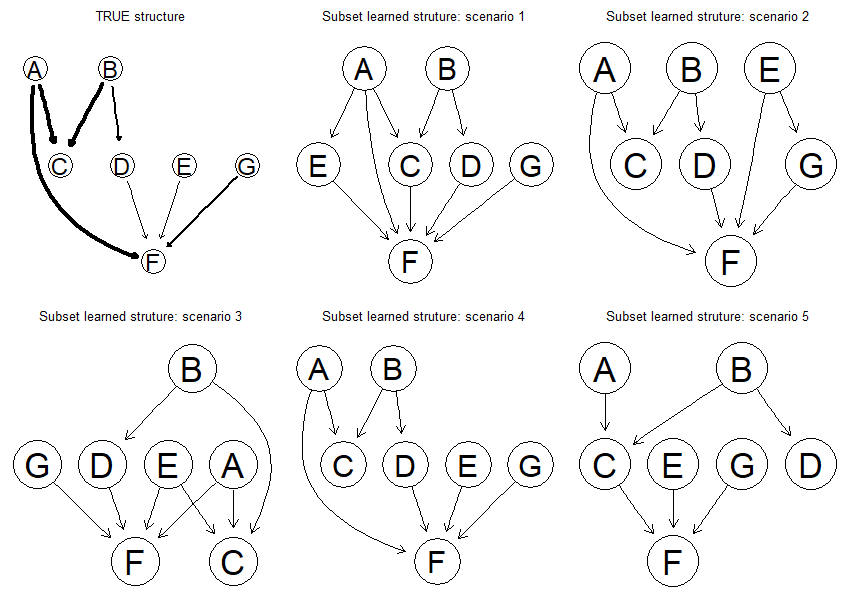
\includegraphics[width=5.34in,height=3.77in]{./media/image2.png}
\end{center}
\vspace{-2.5em}
\vspace{\baselineskip}{\fontsize{8pt}{10.8pt}\selectfont Figure 2: True structure and subset learned structures for the simulated data. \textit{True structure}: thickness of the arcs indicates how strong the association is between variables. \textit{Subset learned structure}: learned from random sampled subsets of size 50. \par}

%   FIGURE 3
\begin{center}
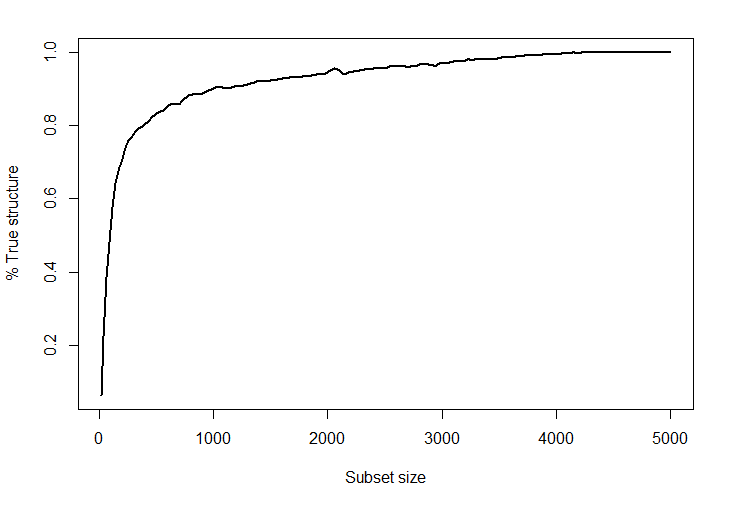
\includegraphics[width=4.59in,height=3.17in]{./media/image3.png}
\end{center}
\vspace{-2.5em}
\vspace{\baselineskip}{\fontsize{8pt}{10.8pt}\selectfont Figure 3: Chance of identifying the true DAG at random sampled subsets of different sizes. }


\subsection{Prediction}
We conduct Bayesian network prediction for variable \textit{F} and compare the performance with traditional multivariate linear regression methods (with all covariates in the model). The prediction error is estimated through cross-validation delete-d (CVd) algorithm. The algorithm randomly selects \textit{d} (in this case use optimal \textit{d}=383) samples as validation set and trains the model with the rest of the data points [8,9]. Since the algorithm prefers small training sets, CVd error is usually larger than other type of CV errors. The CVd mean square errors (CVd-MSE) are used as the criteria to evaluate prediction performances. \par

Figure 4 shows the mean MSEs from 1000 simulations under every given training set size. The red line stands for the BN prediction errors using expert network. If we possess precise understanding about the true DAG, then BN method outperforms other methods. As the training sample size increases, the MSE approaches the theoretical variance of outcome, which is the minimum MSE we can achieve (Figure 4, red). If we know nothing about the truth, the BN method predicts poorer than linear regression when the training set is small (\textit{n}$<$100). However, under larger training sets, BN beats the traditional linear regression methods (Figure 4, blue $\&$ black). \par

Furthermore, we exhaustively fit all possible linear models and identify the model with best prediction performance (using $``$bestglm" package). This model successfully includes all the effective predictors (\textit{A}, \textit{D}, \textit{E}, \textit{G}) of outcome \textit{F} (as shown in expert DAG), and yields equivalent prediction errors as BN. However, the exhaustive algorithm is much more time-consuming. \par

Therefore, the prediction performance of Bayesian networks depends on two factors: 1. More prior knowledge leads to more detailed and precise DAG and yields better prediction. 2. Larger size of training set can ensure the identification of true DAG, also provides more accurate estimates of the parameters in the Bayesian model (especially when the network is complicated). \par

%   FIGURE 4
\begin{center}
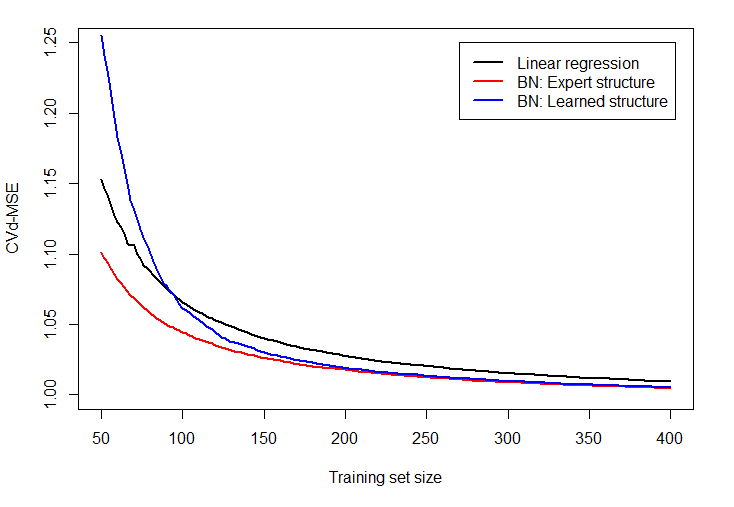
\includegraphics[width=4.59in,height=3.17in]{./media/image4.png}
\end{center}
\vspace{-2.5em}
\vspace{\baselineskip}{\fontsize{8pt}{10.8pt}\selectfont Figure 4: CVd-MSE using different set of training set. Black: linear regression with all variables. \textit{Red}: Bayesian network prediction using true DAG. \textit{Blue}: Bayesian network prediction using DAG learned from training set. \par}




%%%   HEART DISEASE DATASET   %%%%%%%%%%%%%%%%%%%%%%%%%%%%%%
\section{HEART DISEASE DATASET}

\subsection{Material and method}
The data are taken from a larger dataset, described by Rousseauw et al, 1983, South African Medical Journal [10], with 462 observations and 9 variables (including the outcome). The outcome of interest is the diagnosis of Coronary Heart Disease (CDH, coded as\textit{ chd}) ascertained by medical records. \par

\vspace{\baselineskip}
Patients’ characteristics are summarized in Table 1. Out of 462 patients, 160 (34.6$\%$) have CHD, and 302 (65.4$\%$) are free of CHD. All exposures are continuous except for family CHD history (\textit{famhist}) with 1 stands for $``$present" and 0 for $``$absent". Tobacco use (\textit{tobacco}) is measured by cumulative tobacco (kg) in lifetime. Type A behavior (\textit{typea}) is measured using Bornter’s short score [16] ranging from 12 to 84 with higher score indicating more hostile, competitive personalities. Other covariates include continuous age (\textit{age}), obesity measured by BMI (\textit{obesity}), current alcohol use (\textit{alcohol}), level of low density lipoprotein cholesterol (\textit{ldl}), and systolic blood pressure (\textit{sbp}). The distributions of covariates are different between CHD and non-CHD groups (Table 1). \par

%   TABLE 1
\begin{center}
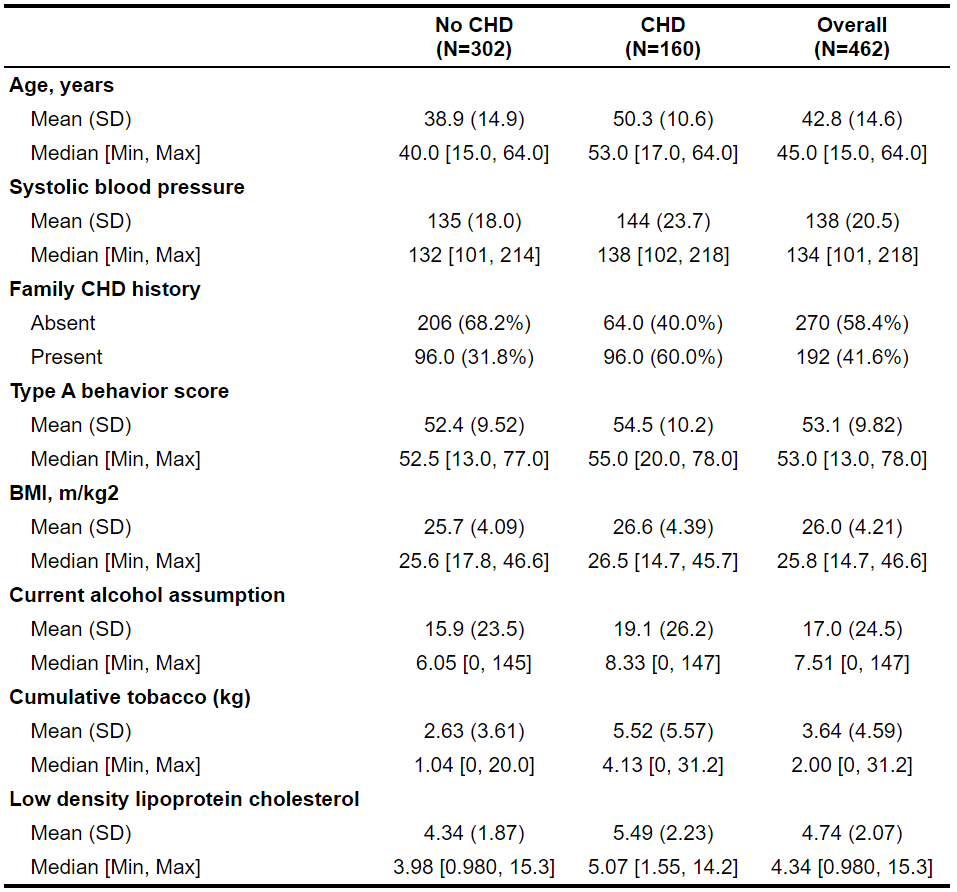
\includegraphics[width=4.98in,height=4.64in]{./media/image5.png}
\end{center}
\vspace{-2.5em}
\vspace{\baselineskip}{\fontsize{8pt}{10.8pt}\selectfont Table 1: Patients’ characteristics by coronary heart disease diagnosis in South African adults. \par}


\subsection{Structure learning}
By computing the covariance matrix, the covariates are highly correlated with each other, implying complicated network structure of the dataset. The structures are learned in the full dataset using both Inter-IAMB and HC algorithms. \par

Prior knowledge from literature review are incorporated into the whitelist (Figure 5, blue arcs): 
\vspace{-1.5em}
\begin{enumerate}
\setlength\itemsep{0em}
\setlength\itemindent{-1em}
	\item High blood pressure [11] and elevated LDL levels [12] are believed to be risk factors and often precedes a diagnosis of CHD.
	\item Alcohol abuse are reported to be associated with escalated SBP [13] and LDL levels [14,15]. 
	\item Obesity adults are more likely to have high SBP [22] and LDL levels [23,24].  
	\item Age is correlated to tobacco use since the latter is measured as lifetime cumulative tobacco use. 
	\item Type A behavior is a valid predictor of CHD risk [16,17]. 
	\item Family history is a strong risk factor of CHD reported in multiple studies [18-20]. 
\end{enumerate} \par

Besides, we forbit some relations and specify the blacklist: 
\vspace{-1.5em}
\begin{enumerate}
\setlength\itemindent{-1em}
\setlength\itemsep{0em}
	\item The exposures were ascertained before the onset of CHD, thus we prevent any arrows starting from \textit{chd }due to temporality. 
	\item Aging (\textit{age}) is a natural process that cannot be the downstream of an arc. 
	\item Family CHD history (\textit{famhist}) is also unlikely to be affected by other covariates.
\end{enumerate} \par

The two algorithms return very similar DAGs as shown in Figure 5. Actually, the only difference is that the inter-IAML algorithm believes that older age leads to increasing Type A behaviors (Figure 5, orange arcs). The DAG implies that age is a potential confounder since it is related to most of the covariates as well as the outcome. Tobacco use has direct effects on CHD even after accounting for the \textit{tobacco}–\textit{alcohol}–\textit{sbp}/\textit{ldl}–\textit{chd} causal pathway. The effects of alcohol use obesity are mediated by blood pressure and LDL levels. \par

We define the HC-learned network (Figure 5, left) as the $``$expert structure" (compared to the structure learned from training sets) and use it for prediction. \par

%   FIGURE 5
\begin{center}
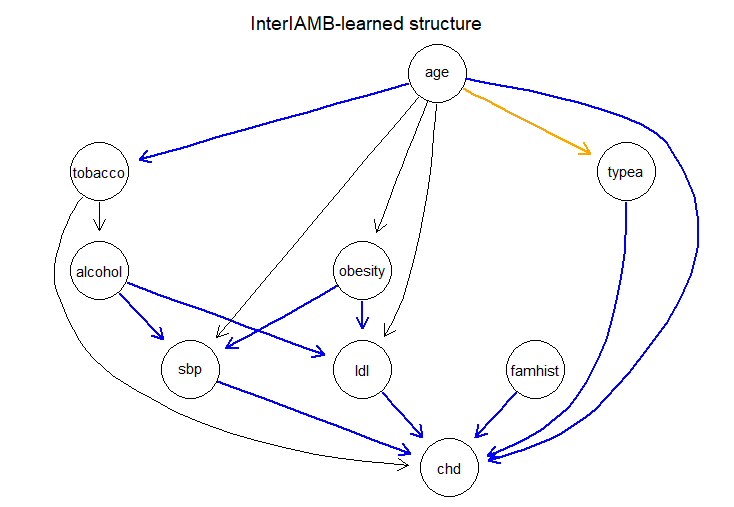
\includegraphics[width=0.45\textwidth]{./media/image6.png}
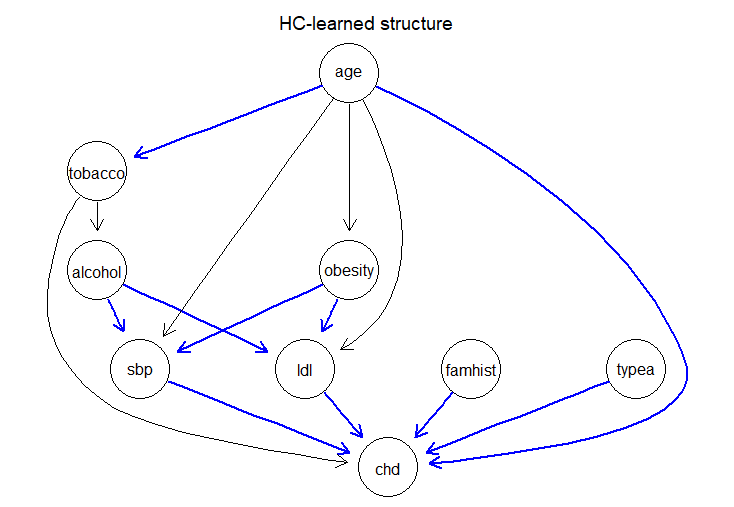
\includegraphics[width=0.45\textwidth]{./media/image7.png}
\end{center}
\vspace{-1em}
{\fontsize{8pt}{10.8pt}\selectfont Figure 5: Structure learning results in CHD dataset. \textit{Blue}: arcs incorporated in the whitelist. These relations always present during structure leaning. \textit{Orange}: disagreement among two algorithms. \par}


\subsection{Best logistic model}
We want to find a traditional frequentist model for comparison. By fitting all covariates into univariate logistic models, we find that all individual variables significantly increase the risk of CHD. In order to directly view their associations, we construct locally Lowess-smoothed scatterplots against the outcome and discover that some effects may not be linear (Figure 6). Thus, we decide to include the quadratic terms for \textit{alcohol}, \textit{tobacco}, \textit{obesity}, and \textit{sbp}. Furthermore, interactions between covariates are tested pairwise. Potential interactions between \textit{sbp} $\&$ \textit{typea}, and \textit{alcohol} $\&$ \textit{obesity}, have been identified. \par

First, we center and scale all continuous covariates including quadratic terms and interactions. Then, an exhaustive strategy is adopted to identify the best logistic prediction model by directly comparing prediction error among all possible models (using BIC as selection criteria yields the same best model). The prediction error is estimated through cross-validation delete-d (CVd) algorithm with optimal \textit{d}=383. We repeat the algorithm 1000 times for each model and pick one model with the lowest mean test error. The best logistic model includes the following predictors: age, tobacco use, Type A score, family history, and LDL level. Note that the expert DAG identifies predictors as \textit{age}, \textit{tobacco}, \textit{typea}, \textit{famhist}, \textit{ldl}, and \textit{sbp}, which almost matches the best logistic predictors. \textit{sbp} is not considered as predictor in the logistic model since it shares the same pathway with \textit{tobacco} (Figure 5).  \par

%   FIGURE 5
\begin{center}
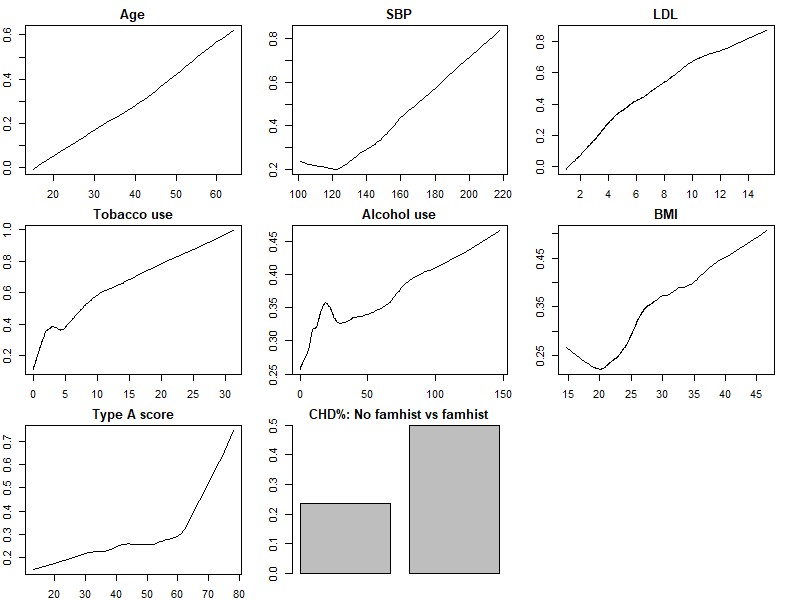
\includegraphics[width=4.87in,height=3.65in]{./media/image8.png}
\end{center}
\vspace{-2.5em}
\vspace{\baselineskip}{\fontsize{8pt}{10.8pt}\selectfont Figure 5: Effects of covariates on CHD diagnosis displayed by locally Lowess-smoothed curves. }


\subsection{Prediction performance}
Since the $``$bnlearn" package doesn’t support estimation for binary outcomes with continuous parent nodes. We treated \textit{chd} as continuous, and BN provides real-valued scores with higher values indicating higher risk of CHD. Area under the curve of ROC (AUC) is used to quantile the discrimination power across two groups. The AUC measures the following property of a classifier: if randomly take one sample from both groups, what’s the probability that the one from the positive outcome group has the higher score? AUC=100$\%$ means that the two groups are totally separated. That is, all cases have higher scores than controls. AUC=50$\%$ suggests that the two groups are mixed by pure randomness [21]. \par

Three prediction models have been brought into comparison: best logistic model, BN with expert structure, BN with structure learned from training sets. Note that in the last method, the structure is learned with only blacklist specified – no prior knowledge (whitelist) being incorporated. \par

Figure 6 shows the results under different sizes of training sets. Under the given training size, mean AUC is computed out of 1000 iterations. BN with expert DAG outperforms the best logistic model when the training set is sufficiently large (\textit{n}$>$250) (Figure 6, red). Under small training set, the best logistic model has the top performance, since it has the fewest parameters to be estimate (Figure 6, black). Without prior knowledge, the BN methods turn out to be the least effective classifiers (Figure 6, blue). If we render the whitelist in the last method, the blue line is expected to be closer to the red line, suggesting a crucial role for prior knowledge when conducting BN prediction. \par

%   FIGURE 6
\begin{center}
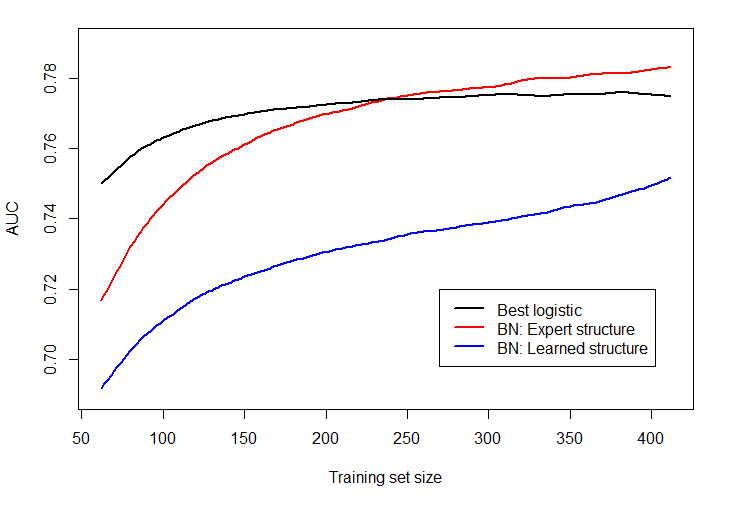
\includegraphics[width=4.59in,height=3.17in]{./media/image9.png}
\end{center}
\vspace{-2.5em}
\vspace{\baselineskip}{\fontsize{8pt}{10.8pt}\selectfont Figure 6: Classification power measured by AUC under different sizes of training sets. \textit{Black}: best logistic model with selected variables. \textit{Red}: Bayesian network prediction using expert DAG. \textit{Blue}: Bayesian network prediction using DAG learned from training set without incorporation of prior knowledge.\par}





%%%   DISCUSSION   %%%%%%%%%%%%%%%%%%%%%%%%%%%%%%
\section{DISCUSSION}

In this study, we compare the prediction performance of Bayesian network with traditional frequentist methods, in both simulated and real-world datasets. BN algorithm has the following strengths: 
\vspace{-1.5em}
\begin{enumerate}
\setlength\itemsep{0em}
\setlength\itemindent{-1em}
	\item It is a powerful tool that provides insights into the probabilistic structure among variables. 
	\item BN prediction can surpass the traditional regression methods in both continuous and classification settings with sufficient prior knowledge and enough training data. 
	\item The structure learning algorithm is fast and easy to conduct. Exhaustive search for frequentist models can sometimes generate similar results. However, these strategies are usually extremely time-consuming, or even unrealistic to perform. 
\end{enumerate} \par

In the CHD dataset, mis-specified DAGs or small sample size can significantly reduce the prediction power of BN. Following strategies maybe able to improve the prediction power further: 
\vspace{-1.5em}
\begin{enumerate}
\setlength\itemsep{0em}
\setlength\itemindent{-1em}
	\item Including more variables helps to identify a more accurate and thorough $``$expert DAG$"$ . 
	\item The data is from a retrospective study conducted in 1980s. Additional techniques may be required to detect and tackle the potential misclassification bias in both exposures and responses.
	\item Since the data is part of a larger dataset, using the whole dataset with greater sample size is expected to refine the prediction by BN algorithm. 
\end{enumerate} \par




%%%   REFERENCE   %%%%%%%%%%%%%%%%%%%%%%%%%%%%%%
\section{REFERENCE}


{\fontsize{8pt}{10.8pt}\selectfont [1] Herskovits, E. (1991). Computer-based probabilistic-network construction (Doctoral dissertation, Stanford University).\par}
\vspace{-1em}
{\fontsize{8pt}{10.8pt}\selectfont [2] Korb, K. B., $\&$  Nicholson, A. E. (2010). Bayesian artificial intelligence. CRC press.\par}
\vspace{-1em}
{\fontsize{8pt}{10.8pt}\selectfont [3] Thulasiraman, K., $\&$  Swamy, M. N. S. (1992). 5.7 acyclic directed graphs. Graphs: theory and algorithms, 118.\par}
\vspace{-1em}
{\fontsize{8pt}{10.8pt}\selectfont [4] Scutari, M. (2009). Learning Bayesian networks with the bnlearn R package. arXiv preprint arXiv:0908.3817.\par}
\vspace{-1em}
{\fontsize{8pt}{10.8pt}\selectfont [5] Pearl, J. (1988). Probabilistic Reasoning in Intelligent Systems: Networks of Plausible Inference Morgan Kaufmann, San Mateo, California 19882. Guttman EA Suchman PF Lazarfeld SA Star and JA Classen Wiley New York 1966.\par}
\vspace{-1em}
{\fontsize{8pt}{10.8pt}\selectfont [6] Verma, T., $\&$  Pearl, J. (1991). Equivalence and synthesis of causal models Proceedings of the Sixth Annual Conference on Uncertainty in Artificial Intelligence.\par}
\vspace{-1em}
{\fontsize{8pt}{10.8pt}\selectfont [7] Chickering, D. M. (1995). A new characterization of equivalent Bayesian network structures. Submitted for publication.\par}
\vspace{-1em}
{\fontsize{8pt}{10.8pt}\selectfont [8] Shao, Jun (1993). Linear Model Selection by Cross-Validation. Journal of the American Statistical Assocation 88, 486-494.\par}
\vspace{-1em}
{\fontsize{8pt}{10.8pt}\selectfont [9] Shao, J. (1997). An asymptotic theory for linear model selection. Statistica sinica, 221-242.\par}
\vspace{-1em}
{\fontsize{8pt}{10.8pt}\selectfont [10] Rossouw, J. E., Du Plessis, J. P., Benadé, A. J., Jordaan, P. C., Kotze, J. P., Jooste, P. L., $\&$  Ferreira, J. J. (1983). Coronary risk factor screening in three rural communities. The CORIS baseline study. South African medical journal= Suid-Afrikaanse tydskrif vir geneeskunde, 64(12), 430-436.\par}
\vspace{-1em}
{\fontsize{8pt}{10.8pt}\selectfont [11] Khot, U. N., Khot, M. B., Bajzer, C. T., Sapp, S. K., Ohman, E. M., Brener, S. J., ... $\&$  Topol, E. J. (2003). Prevalence of conventional risk factors in patients with coronary heart disease. Jama, 290(7), 898-904.\par}
\vspace{-1em}
{\fontsize{8pt}{10.8pt}\selectfont [12] Manninen, V., Tenkanen, L., Koskinen, P., Huttunen, J. K., Mänttäri, M., Heinonen, O. P., $\&$  Frick, M. H. (1992). Joint effects of serum triglyceride and LDL cholesterol and HDL cholesterol concentrations on coronary heart disease risk in the Helsinki Heart Study. Implications for treatment. Circulation, 85(1), 37-45.\par}
\vspace{-1em}
{\fontsize{8pt}{10.8pt}\selectfont [13] Foerster, M., Marques-Vidal, P., Gmel, G., Daeppen, J. B., Cornuz, J., Hayoz, D., ... $\&$  Rodondi, N. (2009). Alcohol drinking and cardiovascular risk in a population with high mean alcohol consumption. The American journal of cardiology, 103(3), 361-368.\par}
\vspace{-1em}
{\fontsize{8pt}{10.8pt}\selectfont [14] Castelli, W., Gordon, T., Hjortland, M., Kagan, A., Doyle, J., Hames, C., ... $\&$  Zukel, W. (1977). Alcohol and blood lipids: the cooperative lipoprotein phenotyping study. The Lancet, 310(8030), 153-155.\par}
\vspace{-1em}
{\fontsize{8pt}{10.8pt}\selectfont [15] Choudhury, S. R., Ueshima, H., Kita, Y., Kobayashi, K. M., Okayama, A., Yamakawa, M., ... $\&$  Miyoshi, Y. (1994). Alcohol intake and serum lipids in a Japanese population. International journal of epidemiology, 23(5), 940-947.\par}
\vspace{-1em}
{\fontsize{8pt}{10.8pt}\selectfont [16] Bortner, R. W. (1969). A short rating scale as a potential measure of pattern A behavior. Journal of chronic diseases, 22(2), 87-91.\par}
\vspace{-1em}
{\fontsize{8pt}{10.8pt}\selectfont [17] Jenkins, C. D., Rosenman, R. H., $\&$  Zyzanski, S. J. (1974). Prediction of clinical coronary heart disease by a test for the coronary-prone behavior pattern. New England Journal of Medicine, 290(23), 1271-1275.\par}
\vspace{-1em}
{\fontsize{8pt}{10.8pt}\selectfont [18] Pohjola-Sintonen, S., Rissanen, A., Liskola, P., $\&$  Luomanmäki, K. (1998). Family history as a risk factor of coronary heart disease in patients under 60 years of age. European heart journal, 19(2), 235-239.\par}
\vspace{-1em}
{\fontsize{8pt}{10.8pt}\selectfont [19] Leander, K., Hallqvist, J., Reuterwall, C., Ahlbom, A., $\&$  de Faire, U. (2001). Family history of coronary heart disease, a strong risk factor for myocardial infarction interacting with other cardiovascular risk factors: results from the Stockholm Heart Epidemiology Program (SHEEP). Epidemiology, 215-221.\par}
\vspace{-1em}
{\fontsize{8pt}{10.8pt}\selectfont [20] Tada, H., Melander, O., Louie, J. Z., Catanese, J. J., Rowland, C. M., Devlin, J. J., ... $\&$  Shiffman, D. (2016). Risk prediction by genetic risk scores for coronary heart disease is independent of self-reported family history. European heart journal, 37(6), 561-567.\par}
\vspace{-1em}
{\fontsize{8pt}{10.8pt}\selectfont [21] Fawcett, T. (2006). An introduction to ROC analysis. Pattern recognition letters, 27(8), 861-874.\par}
\vspace{-1em}
{\fontsize{8pt}{10.8pt}\selectfont [22] Maggio, A. B., Aggoun, Y., Marchand, L. M., Martin, X. E., Herrmann, F., Beghetti, M., $\&$  Farpour-Lambert, N. J. (2008). Associations among obesity, blood pressure, and left ventricular mass. The Journal of pediatrics, 152(4), 489-493.\par}
\vspace{-1em}
{\fontsize{8pt}{10.8pt}\selectfont [23] Couillard, C., Ruel, G., Archer, W. R., Pomerleau, S., Bergeron, J., Couture, P., ... $\&$  Bergeron, N. (2005). Circulating levels of oxidative stress markers and endothelial adhesion molecules in men with abdominal obesity. The Journal of Clinical Endocrinology $\&$  Metabolism, 90(12), 6454-6459.\par}
\vspace{-1em}
{\fontsize{8pt}{10.8pt}\selectfont [24] Weinbrenner, T., Schröder, H., Escurriol, V., Fito, M., Elosua, R., Vila, J., ... $\&$  Covas, M. I. (2006). Circulating oxidized LDL is associated with increased waist circumference independent of body mass index in men and women. The American journal of clinical nutrition, 83(1), 30-35.\par}
\end{document}
%%% TEXT  ENDS  HERE %%%
%%%%%%%%%%%%%%%%%%%%%%%%%%%%%%
